%!TEX root = ../mieic.tex

\chapter{Revisão Bibliográfica} \label{chap:chap2}

\section*{}

\section{Introdução}

Neste capítulo será feita uma análise dos serviços já disponíveis que são relevantes para esta dissertação.
Inicialmente, dar-se-á foco ao RAMA, para depois se comparar as suas funcionalidades com os projetos relacionados.

Esta dissertação foca-se mais na forma como se apresenta o conteúdo que se pretende recomendar ao utilizador, e não qual o conteúdo que é sugerido (não obstante da sua importância obviamente).
No entanto, é quase impossível, no estudo do estado da arte, não se referir outros projetos que se focam também no conteúdo.
Regra geral, os projetos que de seguida serão analisados, utilizam bases de dados externas, como o last.fm, para obter metadata que, convenientemente, também oferecem um tipo de recomendação de música com base numa pesquisa inicial.
Tal não invalida que o tratamento dessa informação seja mal feito, e por isso, será feita uma pequena análise dos conteúdos sugeridos em cada um dos serviços.

\section{RAMA - Relational Artist MAps} % (fold)
\label{sec:rama}

% section rama (end)

\section{Projetos Relacionados} % (fold)
\label{sec:projetos_relacionados}


\subsection{Liveplasma - liveplasma.com} % (fold)
\label{sub:liveplasma}

O liveplasma.com é uma aplicação em flash que mostra relações de artistas de música em forma de grafo, para além de também permitir criar grafos com livros e filmes.
Este não permite editar o grafo e, ao clicar num nó o grafo, é novamente gerado a partir desse nó.

\begin{figure}[tb]
  \begin{center}
    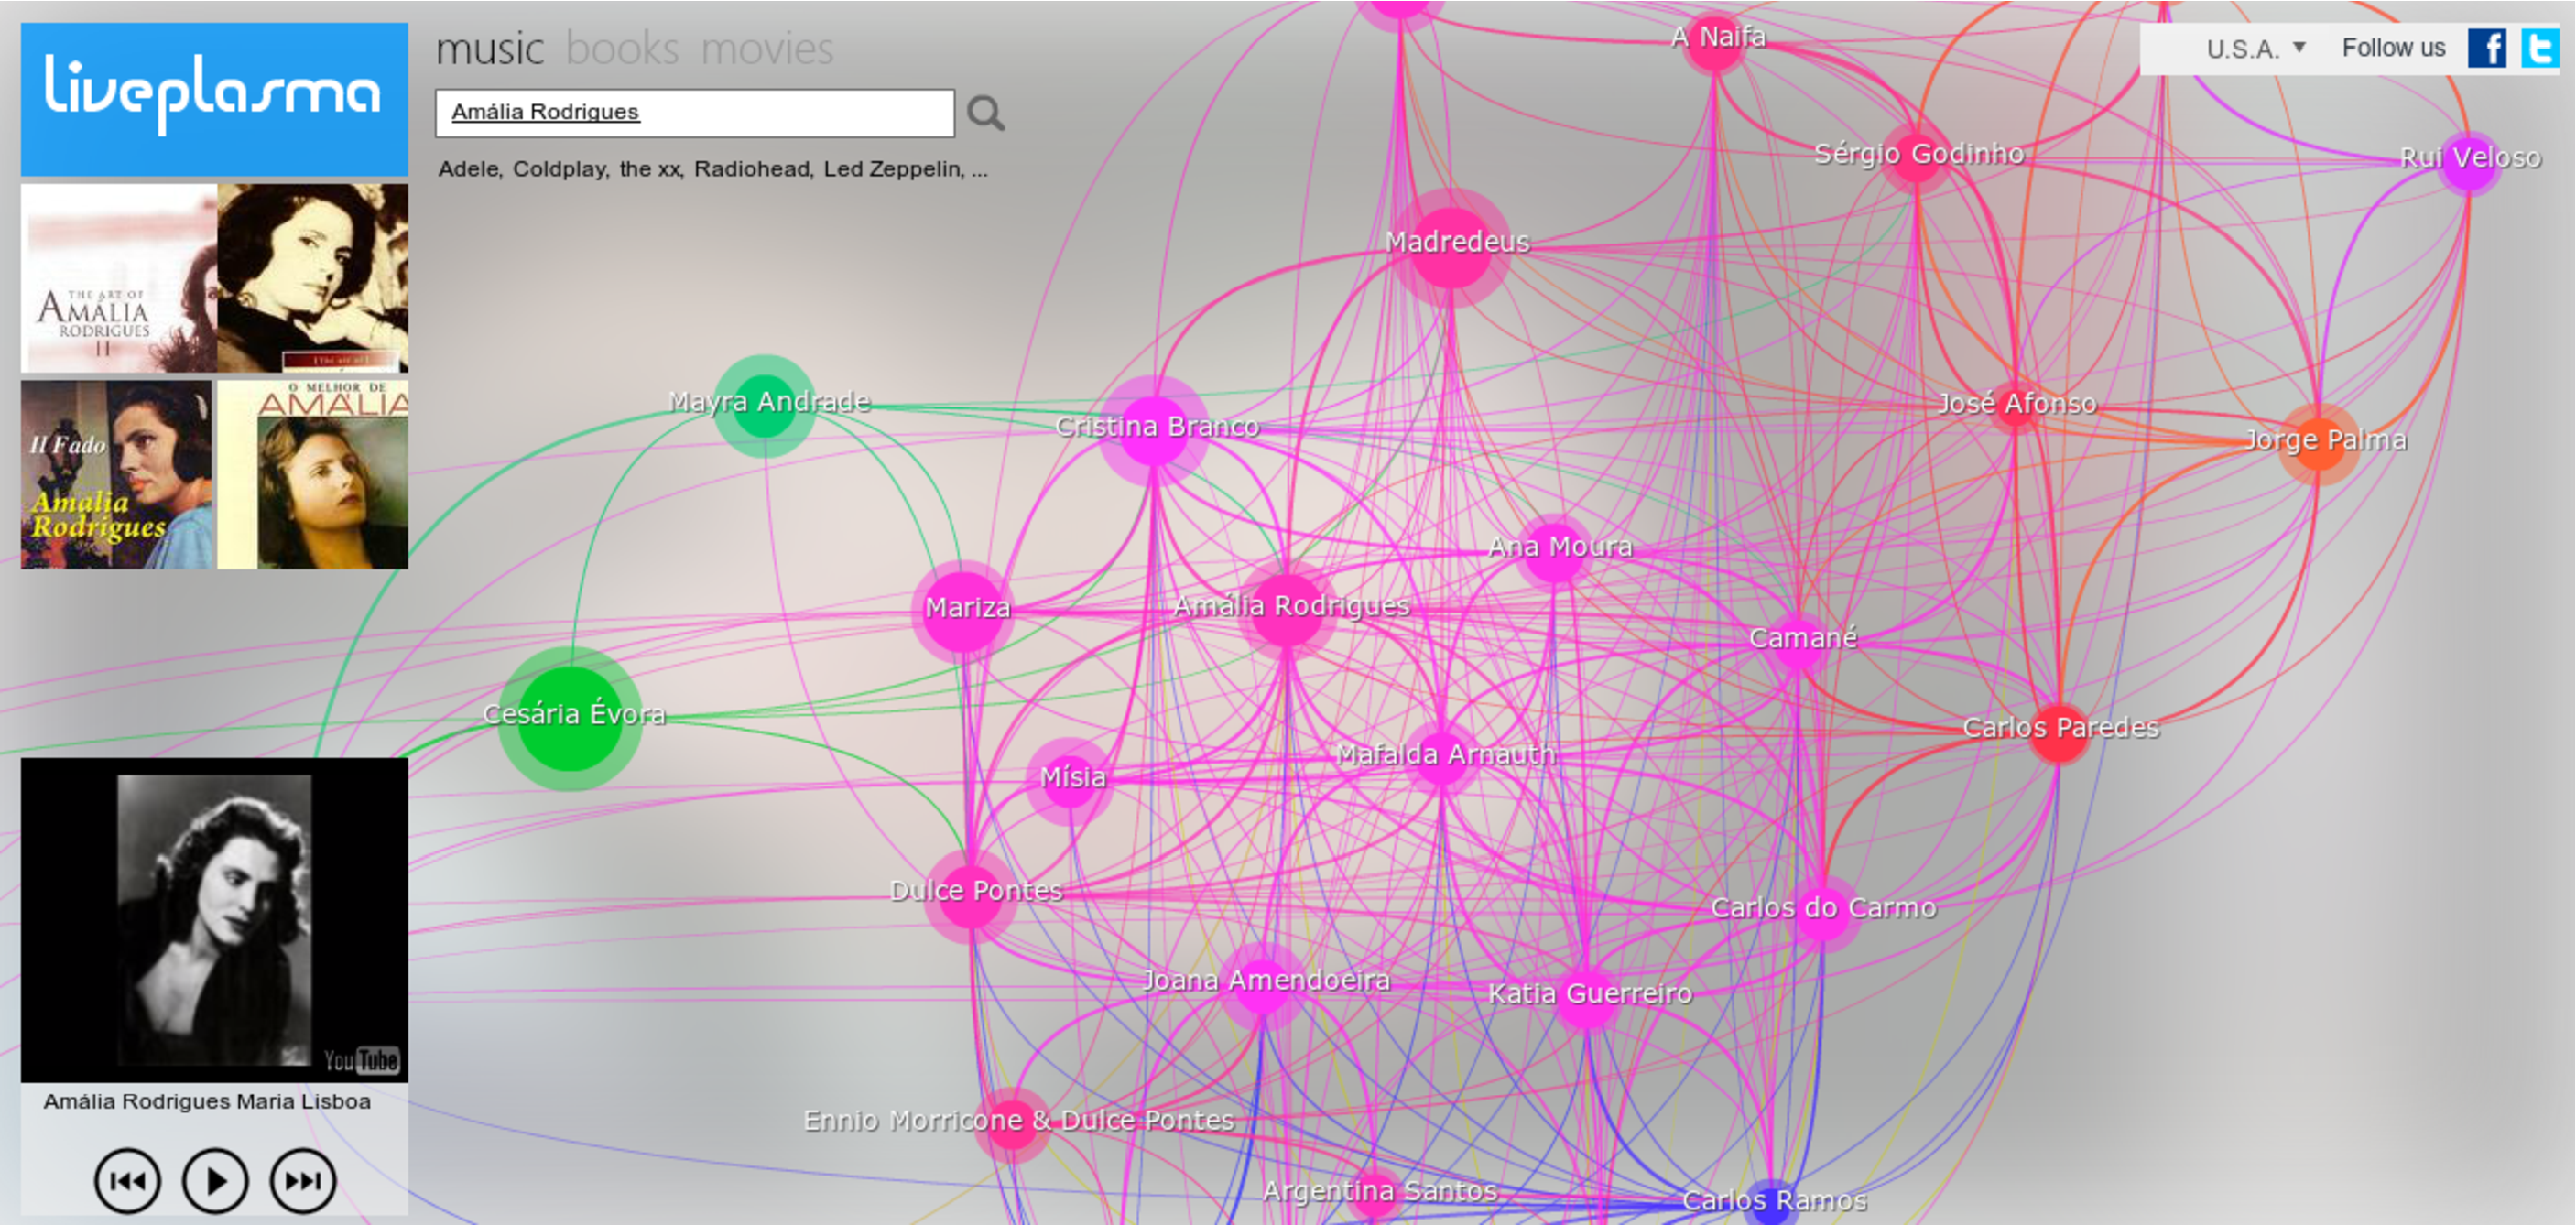
\includegraphics[width=\textwidth]{liveplasma.pdf}
  \end{center}
  \caption{liveplasma: resultado da pesquisa "Amália Rodrigues". Canto superior esquerdo: álbums da artista; Canto inferior esquerdo: \emph{mini-player} do youtube.}
  \label{fig:sota_liveplasma}
\end{figure}

Na figura \ref{fig:sota_liveplasma} podemos ver o resultado de uma pesquisa.
É possível ver a grelha com os álbums que o artista lançou, que redirecionam o utilizador para a Amazon\footnote{http://amazon.com} para comprar os álbums e um \emph{mini-player} que começa a reproduzir uma música do artista diretamente do Youtube.

É possível controlar que músicas são reproduzidas de uma forma interessante: ao passar o rato por cima de um nó, aparece dois botões que permitem reproduzir música só do próprio artista (botão \emph{only}) ou só de artistas parecidos (botão \emph{similar}).
É possível ver esses botões na figura \ref{fig:sota_liveplasma2}

\begin{figure}[tb]
  \begin{center}
    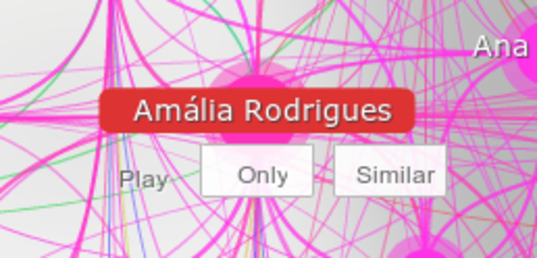
\includegraphics[]{liveplasma2.pdf}
  \end{center}
  \caption{liveplasma: interface para reprodução de música. Botão \emph{similar} reproduz músicas de artistas parecidos; Botão \emph{only} só reproduz músicas do artista pesquisado.}
  \label{fig:sota_liveplasma2}
\end{figure}

\subsubsection{Prós} % (fold)
\label{ssub:liveplasma_pros}

Os aspetos interessantes desta ferramenta são:

\begin{itemize}
  \item Links para compra dos álbums
  \item Reproduzir músicas de artistas semelhantes
\end{itemize}

% subsubsection pros (end)

\subsubsection{Contras} % (fold)
\label{ssub:liveplasma_contras}

O grafo desenhado é bastante confuso quando existem muitos nós com muitas ligações.
Isto acontece quando existem muitos artistas semelhantes.
Para além disso, são atribuídas cores aos nós que devem identificar o grau de parecença entre os artistas.
No entanto não existe nenhum tipo de informação que explique qual o seu verdadeiro significado ao utilizador, assim como também não existe uma explicação das ligações entre os nós.

É também de notar que o tamanho dos nós é diretamente proporcional à popularidade dos artistas respectivos, mas mais uma vez, este tipo de informação não é dada ao utilizador.

Outra falha a apontar é o facto de não se conseguir distinguir o nó de pesquisa dos restantes resultados em \ref{fig:sota_liveplasma} por exemplo.

% subsubsection contras (end)

\subsubsection{Resumo} % (fold)
\label{ssub:liveplasma_resumo}

Em suma, o liveplasma é usável, mas peca por ter muitas cores e ligações que tornam a experiência do utilizador ainda mais difícil do que a tradicional apresentação em lista ou grelha.

% subsubsection resumo (end)

% subsection liveplasma (end)

\subsection{Tuneglue - audiomap.tuneglue.net} % (fold)
\label{sub:tuneglue}

O Tuneglue é outro serviço do mesmo género (também desenvolvido em flash) que usa a base de dados do last.fm para recolher a informação dos artistas de música, assim como artistas relacionados.

Depois da pesquisa de um artista, por exemplo "Mariza", obtemos um grafo com apenas o nó de pesquisa. Ao clicar no nó é apresentado um menu com várias opções como se pode ver na figura \ref{fig:sota_tuneglue}.

\begin{figure}[tb]
  \begin{center}
    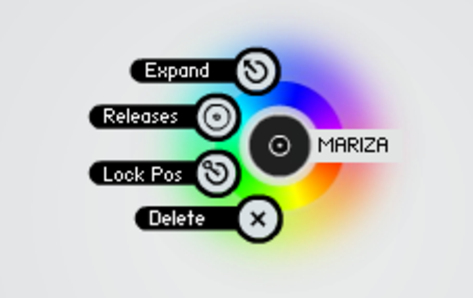
\includegraphics[]{tuneglue.pdf}
  \end{center}
  \caption{Tuneglue: menu que aparece ao clicar num nó.}
  \label{fig:sota_tuneglue}
\end{figure}

A partir deste menu é possível ver uma das principais diferenças que o Tuneglue tem em relação ao liveplasma (\ref{sub:liveplasma}): a edição do grafo.
É possível expandir, fixar e eliminar individualmente cada nó do grafo.
Ao expandir o nó inicial de pesquisa, os nós novos estão apenas e só diretamente relacionados com o nó pai, como se pode ver na figura~\ref{fig:sota_tuneglue2}.

\begin{figure}[tb]
  \begin{center}
    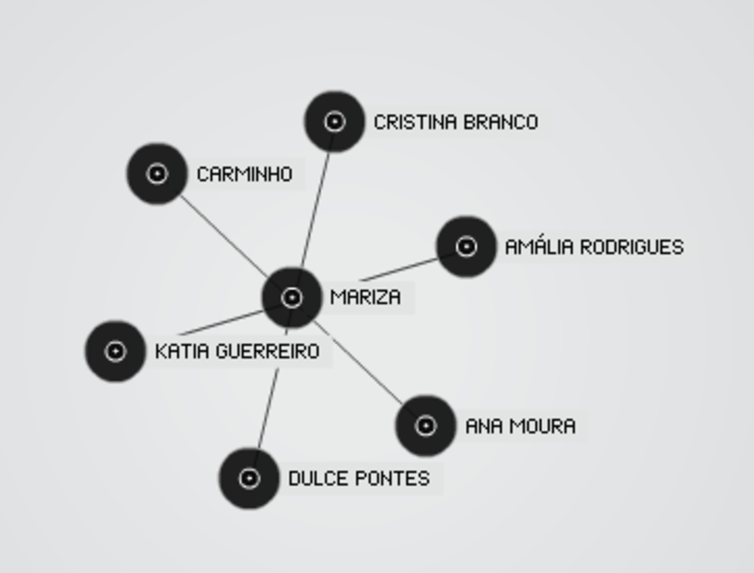
\includegraphics[]{tuneglue2.pdf}
  \end{center}
  \caption{Tuneglue: grafo depois do primeiro nó ser expandido.}
  \label{fig:sota_tuneglue2}
\end{figure}

Ao contrário do Liveplasma, o Tuneglue não faz uma pesquisa recursiva.

\subsubsection{Prós} % (fold)
\label{ssub:audiomap_pros}

Dá bastante liberdade ao utilizador, pois dá-lhe toda a responsabilidade na criação do grafo.
O utilizador sente que todo o grafo foi criação sua e dissimula o utilizador a pensar que foi este que descobriu novos artistas ao invés de receber recomendações.

% subsubsection pros (end)

\subsubsection{Contras} % (fold)
\label{ssub:audiomap_contras}

Mais uma vez, o facto da ferramenta ser feita em flash não ajuda a que a interface seja intuitiva.
Para além de pouco responsiva (o utilizador ao início pode-se sentir perdido por não saber o que fazer), é bastante uniforme, ou seja, não salienta diferenças entre cada artista, nem distingue as ligações entre eles.

% subsubsection contras (end)

\subsubsection{Resumo} % (fold)
\label{ssub:audiomap_resumo}

Em suma, o Tuneglue é inteligente por dar poder ao utilizador, mas ao mesmo tempo não existe um limite nesse poder.
E assim, é possível expandir o grafo até se tornar ilegível.



% subsubsection resumo (end)

% subsection tuneglue (end)

\subsection{MusicRoamer - musicroamer.com} % (fold)
\label{sub:musicroamer}

  O MusicRoamer é outra ferramenta que permite explorar música nova.
  Tal como o Tuneglue, este permitir construir o grafo à medida que se expande cada nó.



  \subsubsection{Prós} % (fold)
  \label{ssub:pros}

  
  Umas das funcionalidades interessantes do MusicRoamer são as várias opções de pesquisa (figura~\ref{fig:sota_musicroamer}):
  \begin{description}
    \item[Pesquisa por Artista] \hfill \\
      Tipo de pesquisa mais utilizada
    \item[Pesquisa por \emph{Keyword}] \hfill \\
      Usar palavras-chave como géneros musicais para pesquisar livremente
    \item[Pesquisa por perfil do Last.fm] \hfill \\
      Esta pesquisa gera um grafo para cada artista (os mais ouvidos pelo utilizador)
  \end{description}

  \begin{figure}[tb]
    \begin{center}
      
\includegraphics[width=\textwidth]{musicroamer.pdf}
    \end{center}
    \caption{MusicRoamer: Várias opções de pesquisa. Por artista; por \emph{keyword} e pelo perfil de utilizador do Last.fm}
    \label{fig:sota_musicroamer}
  \end{figure}

  Todas estas formas de pesquisa desenham um (ou mais) grafo(s) em que os nós são sempre artistas de música.

  O que esta ferramenta trás de novo é a forma como apresenta os grafos.
  A figura~\ref{fig:sota_musicroamer3} apresenta o resultado da pesquisa por Artista "Mariza".
  Imagens dos artistas são usadas para representar os nós, o que ajuda o utilizador a diferenciar os resultados.

  A ferramenta também disponibiliza alguns parâmetros de personalização do grafo (figura~\ref{fig:sota_musicroamer2}) como Zoom, Tamanho da repulsão, imagem entre os nós e o número de artistas de música que deve expandir de um nó.

  \begin{figure}[tb]
    \begin{center}
      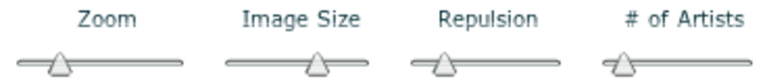
\includegraphics[width=\textwidth]{musicroamer2.pdf}
    \end{center}
    \caption{MusicRoamer: Parâmetros de personalização do grafo}
    \label{fig:sota_musicroamer2}
  \end{figure}



  \begin{figure}[tb]
    \begin{center}
      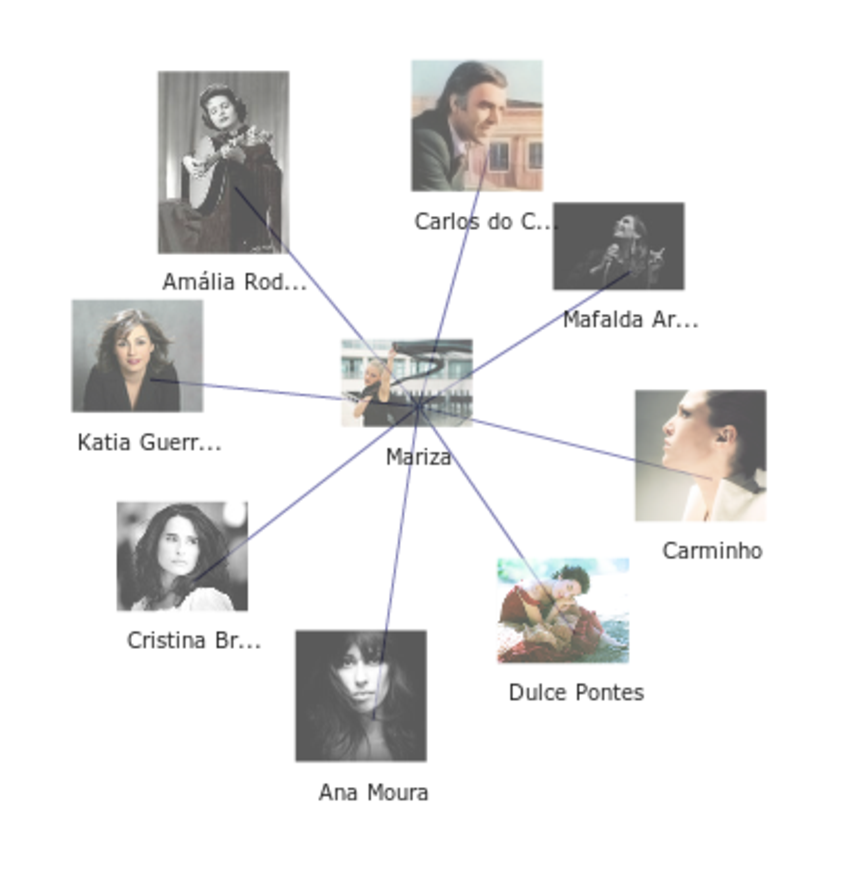
\includegraphics[width=\textwidth]{musicroamer3.pdf}
    \end{center}
    \caption{MusicRoamer: Representação visual do grafo de artistas}
    \label{fig:sota_musicroamer3}
  \end{figure}

  % subsubsection pros (end)

  \subsubsection{Contras} % (fold)
  \label{ssub:contras}

  Um problema do MusicRoamer é o facto de ser feito em flash, pois torna a interface menos natural e fluída.
  Para além disso, à medida que a profundidade do grafo vai aumentando, o grafo começa a ficar confuso e ilegível (figura~\ref{fig:sota_musicroamer4}).
  A linhas começam a se sobrepor e alguns nós ficam pouco legíveis.

  \begin{figure}[tb]
    \begin{center}
      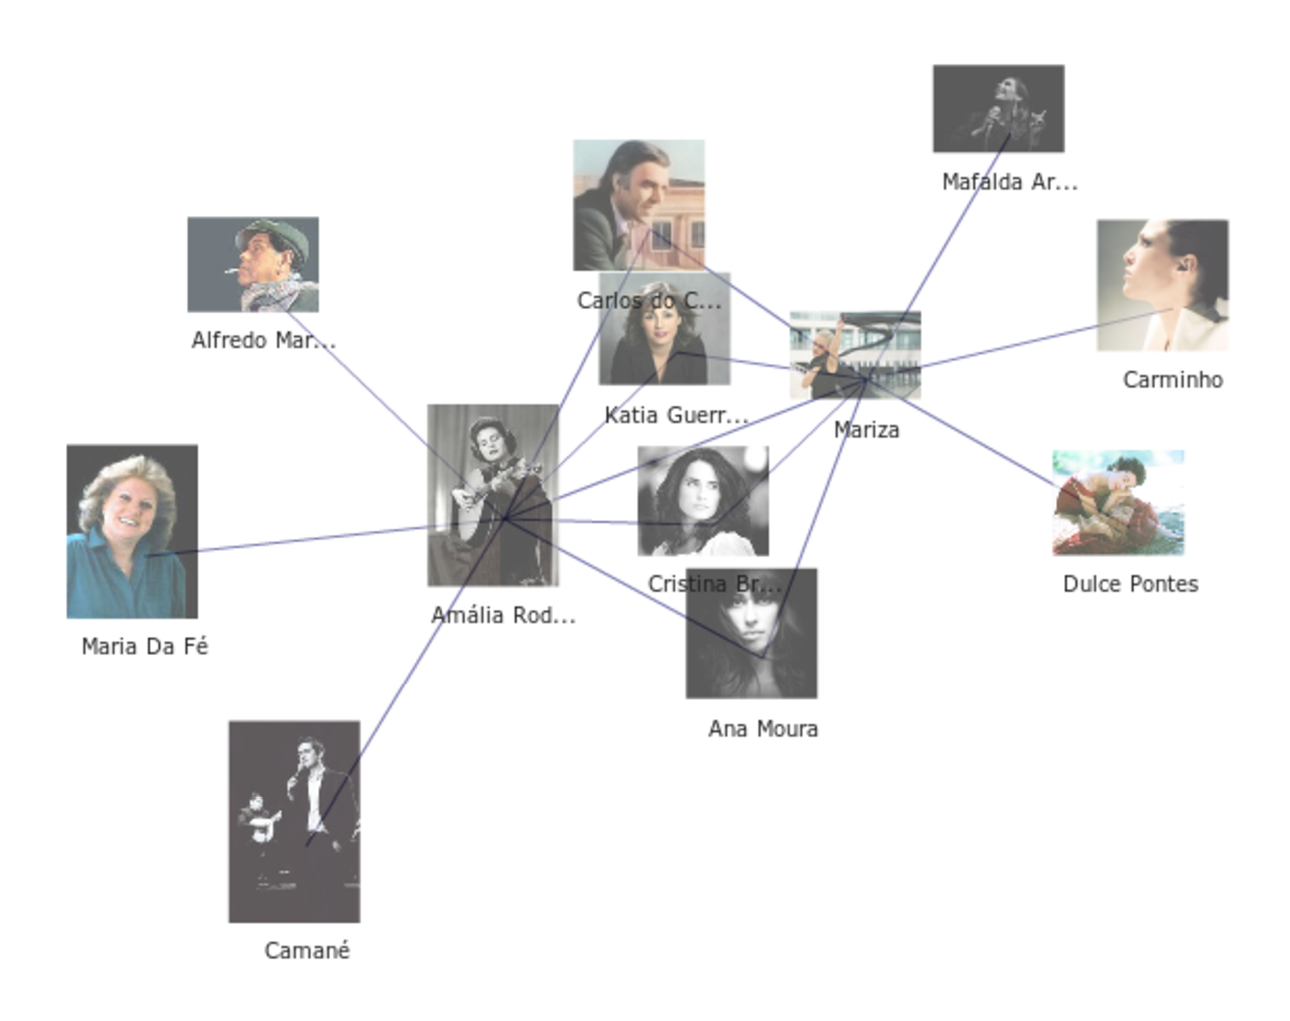
\includegraphics[width=\textwidth]{musicroamer4.pdf}
    \end{center}
    \caption{MusicRoamer: Grafo depois de expandir um nó}
    \label{fig:sota_musicroamer4}
  \end{figure}

  % subsubsection contras (end)

  \subsubsection{Resumo} % (fold)
  \label{ssub:resumo}

  Apesar de um utilizador do MusicRoamer ter muita liberdade na criação do grafo, a sua apresentação global é fraca e pouco trabalhada esteticamente.
  
  % subsubsection resumo (end)

% subsection musicroamer (end)


% section projetos_relacionados (end)


\section{Resumo e Conclusões}

Existem muitas outras ferramentas de descoberta de música. Apesar serem poucas as que usam esta representação visual em grafo, todas elas são importantes de se referir:

\begin{itemize}
  \item liveplasma.com
  \item audiomapa.tuneglue.net
  \item musicroamer.com
  \item discovr.info
  \item ifyoudig.net
  \item pitchfork.com
  \item hypem.com
  \item awdio.com
  \item 8tracks.com
  \item tastekid.com
  \item songza.com
  \item thesixtyone.com
  \item mog.com
  \item stereogum.com
  \item gigfi.com
  \item jango.com
  \item soundcloud.com
  \item grooveshark.com
\end{itemize}


Umas das primeiras lições que se tira dos exemplos dados é que quanto maior for o fator de ramificação de um grafo, mais confuso e saturado se torna.
Não é um exagero dizer que para além de confuso, o grafo perde o seu propósito inicial de ajudar o utilizador na sua descoberta de música nova.

Uma forma de evitar este problema, será limitar o fator de ramificação a um máximo que não cause este problema.

